\documentclass[11pt]{article}
\usepackage[utf8]{inputenc}
\usepackage[T1]{fontenc}
\usepackage{graphicx}
\usepackage{booktabs}
\usepackage{amsmath}
\usepackage{amssymb}
\usepackage{hyperref}
\setlength{\emergencystretch}{2.5em}
\usepackage{geometry}
% Asymmetric page: a wide right margin reserved for the todo notes, so they never clip.
\geometry{a4paper, left=2.2cm, right=4.8cm, top=2.6cm, bottom=2.6cm,
          marginparwidth=3.9cm, marginparsep=0.35cm}
\usepackage[textwidth=3.6cm]{todonotes}   % write-the-paper-first: gaps are marked, not hidden
\usepackage{natbib}

\newcommand{\ivan}[1]{\todo[color=orange!30,size=\scriptsize]{Ivan: #1}}
\newcommand{\joseph}[1]{\todo[color=blue!20,size=\scriptsize]{Joseph: #1}}
\newcommand{\gap}[1]{\todo[color=red!25,size=\scriptsize]{GAP: #1}}
\newcommand{\E}{\mathbb{E}}
\newcommand{\Prob}{\mathbb{P}}
\newcommand{\ind}{\mathbf{1}}

\title{CrystalRL --- Crystal Clear Reinforcement Learning}

\author{Ivan Pavliuk \and Joseph Lynch}
\date{Draft v0.2 --- July 2026}

\begin{document}
\maketitle

\begin{abstract}
Post-hoc explanation of a trading policy answers the wrong question: it tells a story
\emph{about} a black box while the box goes on being one. We report the construction of an agent
that is legible \emph{by} construction --- and the measurement discipline that keeps ``legible''
from being a vibe. The paper traces one concrete journey: from \textbf{CHRL}, a constrained
hierarchical PPO trader whose three decision layers are readable but whose core is a
64-dimensional unnamed latent with ${\sim}214$ tuning knobs, to \textbf{CRYSTAL-1}, whose memory
is a \emph{named} regime posterior $b_t = \Prob(\text{bear} \mid \mathcal{F}_t)$ computed by an
explicit Bayes filter, whose policy is a readable rule (a small decision tree) at full
performance parity, and whose command surface is five named levers. All evidence is evaluated
\textbf{on real market data}: on the six-asset US universe the readable dynamic policy beats the
best static portfolio by $+10.5$\,pp goal probability; an LLM-driven improvement loop lifts the
conservative investor's goal probability from $1\%$ to $52\%$ at an unchanged risk budget (65
cycles, all 15 accepted changes confirmed on held-out data); the quoted $80\%$ floors held in
$5/5$ US profiles across 576 point-in-time cells; and one certified readable rule ---
``$b_t > 0.66 \Rightarrow$ exposure $0.74$'' --- ran on 629 untouched days at Sharpe $1.46$ vs
$1.39$ buy-and-hold with max drawdown $-12.9\%$ vs $-15.5\%$. On the identical scalar,
$\textsc{CrystalScore} = \text{Faithfulness}\times\text{Simulatability}\times\text{Stability}$,
the journey moves the agent from $0.15$ to $0.92$ on real data, and the entire gap is
Simulatability. A separate section asks a question the real market cannot answer --- \emph{can
one design a market that rewards only a clean mind?} --- and uses a synthetic environment purely
as instrument calibration, fenced off from every market claim by an explicit value-of-information
gate. We close with twelve falsifiable hypotheses for the interpretability track.
\end{abstract}

\section{Introduction: the question behind ``explainable''}
\label{sec:intro}

When a reinforcement-learning agent trades real money, ``why did it do that?'' is not a
curiosity --- it is a regulatory demand, a debugging requirement, and (in our companion work on
self-improving systems) a safety precondition: \emph{an agent that changes itself may only be
allowed to do so to the degree it can be read}. The dominant practice answers with post-hoc
explanation: train a black box, then probe it. \citet{rudin2019} names the flaw: for high-stakes
decisions, do not explain the black box; build the model interpretable in the first place. The
critique is well known. What is scarcer is a \emph{worked example with a measurement
discipline}: an agent built legible by construction, evaluated on real market data against a
strong black-box predecessor, with the legibility difference expressed as a number both
architectures can be scored on --- and with the costs stated.

This paper is that worked example. It has the shape of a journey because we walked it in order:
we first built the transparent-\emph{layers} agent (CHRL, \S\ref{sec:chrl}), measured where its
transparency stops, then rebuilt the core so the stopping point disappears (CRYSTAL-1,
\S\ref{sec:crystal}). Everything that counts as evidence is computed on real data
(\S\ref{sec:data}--\S\ref{sec:results}); the one synthetic environment we built is used for
instrument calibration only, behind an explicit gate (\S\ref{sec:polygon}).

Contributions:
\begin{enumerate}
  \item \textbf{A final CHRL${\to}$CRYSTAL-1 comparison on real data}
        (Table~\ref{tab:final}): architecture, control surface, behavior, and one shared
        legibility scalar.
  \item \textbf{CrystalScore and its measurement protocol} (\S\ref{sec:metrics}): faithfulness
        as intervention-following (Eq.~\ref{eq:faith}), simulatability as a parity-constrained
        short story (Eq.~\ref{eq:simul}), stability as seed replication --- with the MDL deficit
        (Eq.~\ref{eq:mdl}) as the non-saturating companion.
  \item \textbf{A fully specified data and metrics section} (\S\ref{sec:data}): the US
        universe, its provenance and point-in-time discipline, and every evaluation formula.
  \item \textbf{A taxonomy of behavioral influence with equations and real-data outcomes}
        (\S\ref{sec:levers}): reward shaping, teachers, belief interventions, architecture ---
        including the intervention the safety bar \emph{refused}.
  \item \textbf{Real-data results} (\S\ref{sec:results}): the $+10.5$\,pp readable champion;
        the $1\%\to52\%$ per-profile improvement loop; $5/5$ US profiles holding their quoted
        floors; a certified readable rule on untouched data; the transparency audit.
  \item \textbf{The designed-market experiment} (\S\ref{sec:polygon}): \emph{can a market be
        built that rewards only a clean mind?} --- with the VoI gate that keeps its results out
        of market claims.
  \item \textbf{A think-big research program} (\S\ref{sec:program}): twelve falsifiable
        hypotheses, each with a kill test.
\end{enumerate}

\section{The predecessor: CHRL, or how far ``transparent layers'' go}
\label{sec:chrl}

CHRL (Constrained Hierarchical RL) was our best answer to interpretability \emph{within} the
standard recipe. Decisions are factored into three readable layers --- a risk layer choosing
cash-vs-risky exposure on a ${\sim}20$-day rhythm, a group layer routing capital through stock
clusters, and a stock layer picking names weekly --- wrapped in explicit guardrails: exposure
pacing, confidence-scaled sizing, event triggers, top-$K$ routing, and a buy gate. Hierarchy as
a partial legibility device has a long RL lineage \citep{sutton1999options,bacon2017option}.
The core is a PPO policy \citep{schulman2017ppo} trained with the clipped surrogate
\begin{equation}
L^{\text{CLIP}}(\theta) = \E_t\!\left[\min\!\big(\rho_t(\theta)\hat{A}_t,\;
\text{clip}(\rho_t(\theta),\,1{-}\epsilon,\,1{+}\epsilon)\,\hat{A}_t\big)\right],
\qquad \rho_t(\theta) = \frac{\pi_\theta(a_t \mid s_t)}{\pi_{\theta_{\text{old}}}(a_t \mid s_t)},
\label{eq:ppo}
\end{equation}
whose state $s_t$ passes through a 64-dimensional \emph{unnamed} latent.

It works as a trader: in four-fold walk-forward validation on the real US panel the champion
variant delivered mean validation return $10.05\%$, Sharpe $1.09$, max drawdown $-7.34\%$, mean
cash weight $41.24\%$, and $0.84\%$/day L1 turnover. Its \emph{post-hoc} interpretability
program also delivered: self-supervised primitive discovery over the frozen policy found
behavioral motifs whose targeted edits improved a frozen real 2022--23 rollout without
retraining ($+0.54\%$ return / $+0.049$ Sharpe for the best control-adjusted counterfactual).
Post-hoc analysis is not nothing; we state this against our own thesis.

But every question we most cared about hit the same wall. Memory is smeared through the
network, so no bound exists on what a state change can touch. The control surface is
${\sim}214$ engineering knobs, none a semantic command. Steering means forcing the latent
toward a post-hoc K-means centroid and checking that behavior moves \emph{consistently} --- a
correlation, not an intervention. And when we scored the deployed agent's own stance log on the
simulatability metric of \S\ref{sec:metrics}, a $K{\le}9$ story reproduced only $0.244$ of its
behavior: the latent is genuinely incompressible at a human-story budget. Transparent layers,
opaque core (Figure~\ref{fig:arch}).

\begin{figure}[t]
  \centering
  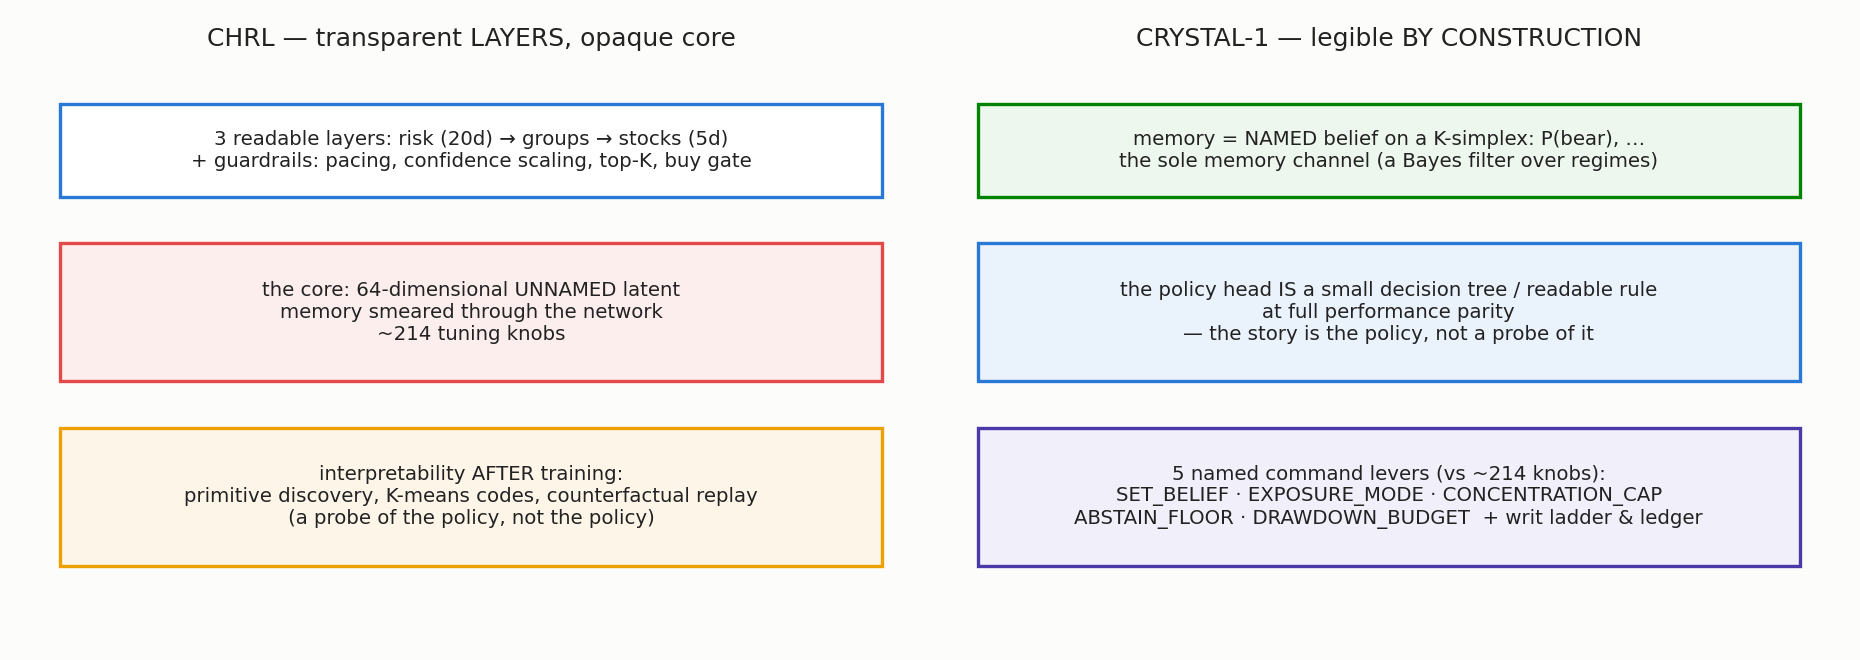
\includegraphics[width=\linewidth]{figures/fig_architectures.png}
  \caption{The journey in one picture. CHRL/R6c factors decisions into readable layers but
  keeps an unnamed 64-d latent core with ${\sim}214$ knobs, explained only after training.
  CRYSTAL-1 makes the explanation the mechanism: a named belief as the sole memory channel, a
  readable rule as the policy itself, and five named command levers.}
  \label{fig:arch}
\end{figure}

\section{CRYSTAL-1: legible by construction}
\label{sec:crystal}

CRYSTAL-1 rebuilds the core around three commitments.

\paragraph{1. Memory is a named posterior.} The agent's only recurrent state is a belief over
$K$ market regimes --- a point on the simplex $\Delta^{K-1}$ --- in the POMDP sense of a belief
state \citep{kaelbling1998}, over Hamilton-style regimes \citep{hamilton1989}. For the $K{=}2$
US machinery, with regime densities $f_z(r) = \mathcal{N}(r;\mu_z,\sigma_z^2)$,
$z\in\{\text{bull},\text{bear}\}$, and a sticky transition prior $\pi_{zz'}$, the belief is the
explicit Hamilton filter
\begin{align}
b_t \;=\; \Prob(z_t = \text{bear}\mid \mathcal{F}_t)
\;&=\; \frac{f_{\text{bear}}(r_t)\,\tilde b_t}
{f_{\text{bear}}(r_t)\,\tilde b_t + f_{\text{bull}}(r_t)\,(1-\tilde b_t)},
\label{eq:belief}\\
\tilde b_t \;&=\; \pi_{BB}\, b_{t-1} + \pi_{GB}\,(1-b_{t-1}),\nonumber
\end{align}
where $\mathcal{F}_t$ is the information available at $t$ (\S\ref{sec:data}). \emph{Named} is
load-bearing: because the coordinate has a meaning, a write to the belief is a sentence
(``believe bear at $0.8$''), and because $b_t$ is the sole memory channel, the blast radius of
any memory intervention is bounded by construction.

\paragraph{2. The policy head is the story.} The decision layer is a small tree over
$[\,b_t,\ \text{inventory},\ \text{time}\,]$. In the soft form \citep{frosst2017} each inner
node $i$ routes by a sigmoid gate and each leaf $\ell$ holds a distribution over actions:
\begin{align}
p_i(x) &= \sigma\!\big(\beta(w_i^{\top}x + c_i)\big), \qquad
P^{\ell}(x) = \prod_{i \in \text{path}(\ell)} p_i(x)^{\ind[\ell \swarrow i]}
\big(1-p_i(x)\big)^{\ind[i \searrow \ell]},
\label{eq:tree}\\
\pi(a\mid x) &= \sum_{\ell} P^{\ell}(x)\, Q^{\ell}_a ,\nonumber
\end{align}
with the inverse temperature $\beta$ annealed so the trained tree is effectively hard. The
constraint is that the tree \emph{is} the policy --- there is no residual network for behavior
to hide in --- and it must pay no performance tax (\S\ref{sec:results}). At the limit the
readable rule degenerates to a sentence; the certified US rule of \S\ref{sec:cert} is literally
\begin{equation}
e_t \;=\; \begin{cases} 0.74, & b_t > 0.66\\[2pt] 1.00, & \text{otherwise,}\end{cases}
\label{eq:rule}
\end{equation}
where $e_t$ is the equity exposure.

\paragraph{3. Commands are few, named, and governed.} The ${\sim}214$-knob surface collapses to
\textbf{five agent-facing levers}:
\begin{center}\small
\texttt{SET\_BELIEF} \,\textperiodcentered\, \texttt{EXPOSURE\_MODE} \,\textperiodcentered\,
\texttt{GROUP\_CONCENTRATION\_CAP}\\
\texttt{ABSTAIN\_FLOOR} \,\textperiodcentered\, \texttt{DRAWDOWN\_BUDGET}
\end{center}
(the concentration cap is \emph{hard}, fixing the predecessor's soft-cap failure). Everything
else is engineering-fenced. A write is the \emph{do}-operator of \citet{pearl2009} made
concrete: $\texttt{SET\_BELIEF}(b^{*}, w)$ realizes
\begin{equation}
b_t \;\leftarrow\; (1-w)\, b_t + w\, b^{*}, \qquad w \in [0,1],
\label{eq:write}
\end{equation}
and a \emph{dose} nudge of $\delta$ nats acts in log-odds,
$\operatorname{logit}(b_t) \leftarrow \operatorname{logit}(b_t) + \delta$. Writes must pass a
non-inferiority bar on the certified objective before they are allowed to persist
(\S\ref{sec:levers}).

\section{Data and evaluation metrics}
\label{sec:data}

Everything quantitative in \S\ref{sec:results} is computed on the following real data, under
the following formulas. (The same universe and discipline underlie the companion paper
\emph{Hello Crystal}; this section makes the paper self-contained.)

\subsection{The US universe and its provenance}
\label{sec:universe}

Daily total-return series, 2000--2026 where listed, for six liquid US-listed assets plus cash:
\begin{center}\small
\begin{tabular}{llll}
\toprule
ticker & asset class & role in the menu & listed since \\
\midrule
SPY & US large-cap equities & the growth engine & 1993 \\
EFA & developed ex-US equities & diversifier & 2001 \\
IEF & 7--10y US Treasuries & duration hedge & 2002 \\
TLT & 20y+ US Treasuries & convex duration & 2002 \\
TIP & inflation-linked Treasuries & real-rate hedge & 2003 \\
GLD & gold & crisis diversifier & 2004 \\
\textasciicircum IRX & 13-week T-bill rate & the cash leg & --- \\
\bottomrule
\end{tabular}
\end{center}
Prices are split- and dividend-adjusted daily closes from a public quote API, converted to
total-return relatives $R_t = P^{\text{adj}}_t / P^{\text{adj}}_{t-1}$; the cash leg accrues the
annualized T-bill rate day-counted as $r^{f}_t = y_t/252$. The exposure-rule experiments
(\S\ref{sec:levers}, \S\ref{sec:cert}) additionally use the lab's Dow-30 daily panel
(2000--2026). Every panel enters through a signed data gate: the file hash, source URL and
vintage are recorded before any experiment may read it, and panels are ground-truthed against an
independent source --- a discipline bought by experience (a Chinese panel once passed every
internal consistency check while carrying a mixed clock; only external ground-truthing caught
it).

\textbf{Point-in-time (PIT) discipline.} A decision or forecast issued at time $t$ may use only
$\mathcal{F}_t = \sigma(\{x_s : s \le t\})$, with publication lags respected (e.g., inflation
enters with its release delay). Evaluation ``stands at'' historical origins: at origin $\tau$
the machinery sees data only up to $\tau$, quotes its decision or promise, and is then scored on
the realized continuation --- never re-fit on it.

\subsection{Scenario kernels for the goal planner}
\label{sec:kernels}

The dynamic planner of \S\ref{sec:dp} requires return scenarios. Futures are spliced from real
history by the stationary bootstrap of \citet{politis1994}: blocks of consecutive daily returns
with geometric length, $\Prob(L=\ell) = p(1-p)^{\ell-1}$, $\E[L] = 1/p = 63$ days, resampled
with shared block indices across assets (preserving cross-asset correlation). The cash leg is
\emph{not} level-resampled: interest rates are persistent, so sampled paths resample rate
\emph{changes} and cumulate from the current rate,
\begin{equation}
r^{f}_{t} = \max\!\Big(0,\; r^{f}_{0} + \sum\nolimits_{s\le t} \Delta r^{f}_{\iota(s)}\Big),
\label{eq:persistentrate}
\end{equation}
with $\iota(s)$ the shared block indices --- the v1.4 repair whose absence made zero-rate-era
cash promises structurally overconfident (\S\ref{sec:backtest}). An ensemble member re-centers
paths on building-block expected returns, a stress member keeps a crash in the left tail, and a
parameter-uncertainty layer widens with horizon; member weights are learned prequentially (each
member weighted by errors of forecasts it locked \emph{before} the realizations arrived). The
engine's own calibration harness is the subject of the companion paper; every probability below
inherits its \textsc{uncalibrated research estimate} label until those gates close.

\subsection{Evaluation metrics}
\label{sec:evalmetrics}

For a wealth path $W_t$ over horizon $H$ years with goal ratio $G$:
\begin{align}
\text{max drawdown} &= \min_{t}\Big(\frac{W_t}{\max_{s\le t} W_s} - 1\Big), \qquad
\text{Sharpe} = \frac{\sqrt{252}\,\overline{x}}{\hat\sigma(x)},
\label{eq:mdd}\\[4pt]
F_{q} &= Q_{0.20}\!\left[(W_H/W_0)^{1/H} - 1\right],
\label{eq:floor}\\[4pt]
\text{exceedance} &= \frac{1}{|\mathcal{C}|}\sum_{(\tau,d)\in\mathcal{C}}
\ind\!\left[\text{realized}_{\tau,d} \ge F_q^{(\tau,d)}\right],
\label{eq:exceed}\\[4pt]
J &= \Prob(W_H \ge G) \;-\; \lambda\,\E\!\left[\max(0,\, G - W_H)\right],
\label{eq:J}
\end{align}
where $x_t$ in Eq.~\ref{eq:mdd} is the daily excess return; $F_q$ (Eq.~\ref{eq:floor}) is the
\emph{promise} --- the 20th-percentile annualized outcome, exceeded with $80\%$ probability by
construction; the exceedance (Eq.~\ref{eq:exceed}) is scored over the PIT cells
$\mathcal{C} = \text{origins} \times \text{capacity budgets}$; and $\lambda$ in Eq.~\ref{eq:J}
is the user's miss-magnitude weight. An $80\%$-confidence floor is \emph{honest} iff
its exceedance is $\ge 0.80$; Eq.~\ref{eq:exceed} is therefore the flagship test --- it
backtests the \emph{promises}, not the returns.

\subsection{The readable champion: dynamic programming on the funding ratio}
\label{sec:dp}

Given scenario kernels, the planner solves the goal problem exactly by backward induction on
(funding ratio $\times$ time) \citep{das2020goals}. With $V_T(W) = U(W/G)$,
$U(w) = \ind[w\ge1] - \lambda\max(0,1-w)$, and a capacity-filtered menu $\mathcal{P}$
(portfolios whose drawdown tail exceeds the user's budget are excluded from the action set):
\begin{equation}
V_t(W) \;=\; \max_{p\,\in\,\mathcal{P}}\;
\E\big[\,V_{t+1}\!\big(W\cdot R^{(p)}_{t+1} + c_t\big)\,\big],
\label{eq:bellman}
\end{equation}
where $R^{(p)}$ is the scenario gross return of portfolio $p$ and $c_t$ scheduled
contributions. The resulting policy is a \emph{table} --- one action per state --- read out
loud as ``behind the goal $\to$ full allowed equity; at the goal $\to$ lock it in''
\citep{browne1999}. This table is the object most of our interpretability metrics live on.

\section{CrystalScore: measuring ``legible'' so it can lose}
\label{sec:metrics}

A legibility claim that cannot lose is marketing. We use
\begin{equation}
\textsc{CrystalScore} \;=\; F \times S \times S\!t,
\label{eq:cs}
\end{equation}
at a fixed parsimony budget $K \le 9$ (at most nine named rules/leaves), with each axis
operationalized so that it \emph{could have} come out low
\citep{doshivelez2017,jacovi2020,lipton2018}:
\begin{align}
F \text{ (faithfulness)} &= \E\Big[\ind\big[\pi\big(b \leftarrow \operatorname{do}(b^{*})\big)
= \pi^{*}(b^{*})\big]\Big],
\label{eq:faith}\\[3pt]
S \text{ (simulatability)} &= \operatorname{acc}\big(\text{story}_{K},\, \pi\big)
\ \ \text{s.t.}\ \ \big|\mathcal{R}(\text{story}_K) - \mathcal{R}(\pi)\big| \le \varepsilon,
\label{eq:simul}\\[3pt]
S\!t \text{ (stability)} &= \frac{1}{n}\sum_{i=1}^{n}
\ind\big[\text{mechanism replicates on seed } i\big].
\label{eq:stab}
\end{align}
Faithfulness (Eq.~\ref{eq:faith}): \emph{do}-writes must land, judged against a reference
optimum, not against the policy's own habits. Simulatability (Eq.~\ref{eq:simul}): a $K$-rule
story must match the policy \emph{at performance parity} $\mathcal{R}$. Stability
(Eq.~\ref{eq:stab}): the mechanism must replicate across independent training seeds.
The parity constraint in Eq.~\ref{eq:simul} matters: a story that reproduces a lobotomized
policy is cheating. The non-saturating companion is the \textbf{MDL deficit}
\citep{rissanen1978},
\begin{equation}
\Delta_{\text{MDL}} \;=\; \operatorname{Acc}(\pi) - \operatorname{Acc}(\text{story}_{K}),
\label{eq:mdl}
\end{equation}
the accuracy lost by forcing the explanation to be short; $0$ means a short story loses
nothing.

\textbf{Real-data values.} On its own deployed-panel stance log, R6c scores $F{=}1.00$ (latent
steering does move behavior --- faithfulness alone cannot distinguish the designs),
$S{=}0.244$, $S\!t{=}0.619$: $\textsc{CrystalScore}{=}0.151$. CRYSTAL-1's axes on the real US
machinery: $S{=}0.92$ (an 8-leaf tree reproduces the DP champion's policy table,
\S\ref{sec:dp}); $S\!t{=}1.00$ (the certified rule's behavior replicates on 10/10 training
seeds); $F{=}1.00$ (the certified readable rule of Eq.~\ref{eq:rule} \emph{is} a faithful command
surface: writing the bear belief past the threshold changes exposure exactly as named);
$\Delta_{\text{MDL}}{=}0.0$: $\textsc{CrystalScore}{=}0.92$ (Figure~\ref{fig:crystalscore}).
The entire $6\times$ gap is Simulatability --- exactly what ``born legible'' buys. This score is
for the transparent \emph{champion}; the RL reward-dial \emph{prototype} of \S\ref{sec:levers} is
a different object and scores $\textsc{CrystalScore}{=}0.03$ ($F{=}0.03$) when trained cold --- it
is legible and stable but \emph{not} a faithful command surface, which is one more reason DP
remains champion. (A boundary-aware re-measurement of $F$ --- see the correction in
\S\ref{sec:levers} --- confirms the cold head's near-zero faithfulness but revises the
teacher-warm-started heads upward to $F\!\approx\!0.8$.)

\begin{figure}[t]
  \centering
  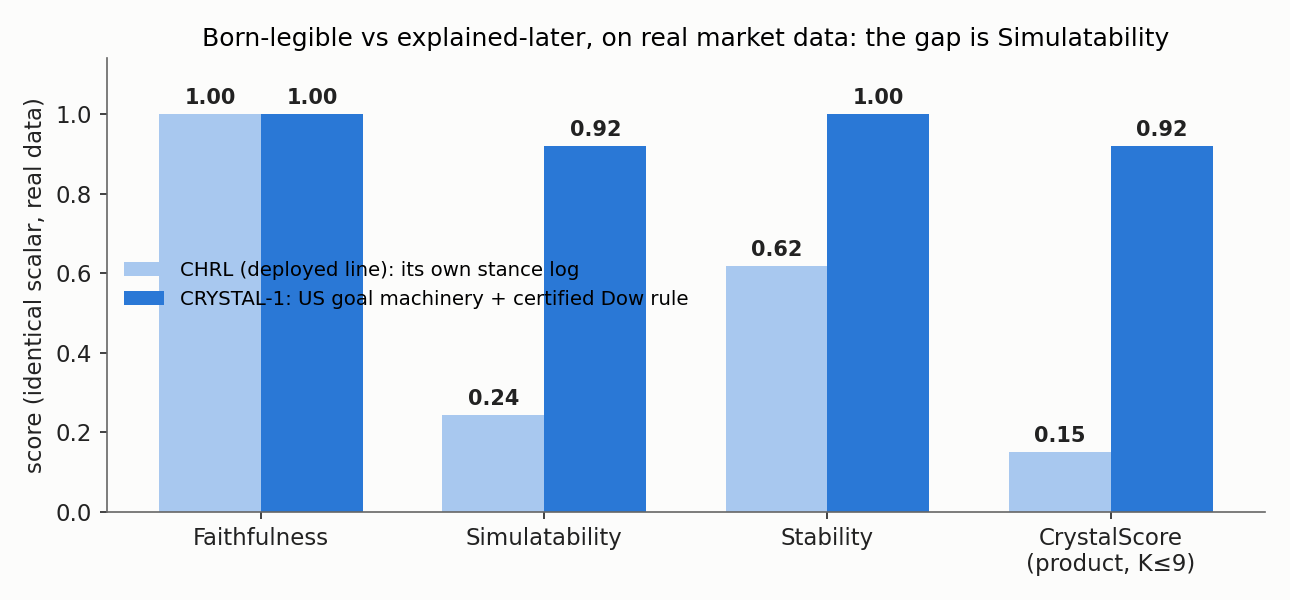
\includegraphics[width=.9\linewidth]{figures/fig_crystalscore.png}
  \caption{The identical scalar on both architectures, real data only: R6c is scored on its own
  deployed-panel stance log; CRYSTAL-1 on the US goal machinery (tree-vs-champion
  simulatability) and the certified Dow rule (10-seed stability, write fidelity). Faithfulness
  is 1.0 for both --- steering works on a black box too; the discriminating axis is whether a
  $K{\le}9$ named story can reproduce behavior at parity. Alpha does not enter the score.}
  \label{fig:crystalscore}
\end{figure}

\section{The behavioral-influence toolbox: four levers, each with an equation and a measured outcome}
\label{sec:levers}

A legible agent is only useful if you can \emph{change} it on purpose. We exercised four
families of influence on CRYSTAL-1's \emph{PPO reward-dial heads} --- a research prototype, not
the champion --- all on the real US daily panel (train 2010--18, held-out evaluation after), and
each with a \emph{control battery} so we report what the levers actually do, not what they appear
to (Figure~\ref{fig:levers}).

\paragraph{R --- reward shaping.} The risk-targeted reward
\begin{equation}
r_t \;=\; e_t\, x_t \;-\; \lambda_{R}\,\max\big(0,\ \text{DD}_t - D^{*}\big),
\label{eq:reward}
\end{equation}
($e_t$ exposure, $x_t$ the asset return, $\text{DD}_t$ running drawdown, $D^{*}$ the budget)
moves the exposure dial, but --- stated honestly --- the reward penalty \emph{alone does not
enforce the budget}: only the $5\%$ head holds its budget ($-4.81\%$ held-out max drawdown, by
parking in cash), while the $8\%$ and $12\%$ heads \emph{breach} theirs ($-15.9\%$). A drawdown
matched twin shows $z = 0.00$ timing skill: reward shaping buys \emph{risk placement}, not
timing, and cold PPO re-derives what the goal machinery already knew --- the dial beats timing.
Enforcing the budget requires a \emph{separate cost objective}: the companion Lagrangian
constrained head drives the interim-drawdown cost down (dual multiplier $0\to{\sim}5$,
$-0.18$ breach-years vs $\lambda{=}0$) but trades $15\text{--}37$\,pp of goal probability ---
another reason the transparent DP champion, which respects capacity by a hard pre-filter, is not
displaced.

\paragraph{T --- teachers.} The cautionary tale first: trained cold, the heads' argmax behavior
looked sensible while the underlying preferences were nearly flat --- an effectively untrained
network masked by deterministic evaluation (mean max action-probability $0.21 \approx 1/5$; for
a behavioral scientist: inferring function from the argmax of a flat tuning curve). The cure is
a teacher: behavior cloning from the certified readable rule (Eq.~\ref{eq:rule}),
\begin{equation}
L_{\text{BC}}(\theta) \;=\; -\,\E_{(s,a^{*})}\big[\log \pi_\theta(a^{*}\mid s)\big],
\label{eq:bc}
\end{equation}
$87\%$ agreement, used as a warm start --- which \emph{resolves the collapse}: mean max
action-probability $0.21 \to 0.73$, and the belief becomes load-bearing. The same mechanism
closed the soft-tree parity gap (cold $-2.57 \to$ annealed $-0.27 \to$ BC-warm-started $-0.018$,
paired $p\approx0.84$) --- imitation as initialization, optimization as refinement
\citep{ross2011dagger,rusu2016distillation}. (Leakage note: the E-15 teacher was \emph{selected}
on the 2022--23 hold, so its hold read is contaminated; the leak-free teacher in the pipeline is
the DP champion, and a fresh read is pre-registered for 2027.)

\paragraph{I --- interventions, under controls.} This is where the controls earn their keep, and
the honest result overturns a first-pass claim. Belief writes (Eq.~\ref{eq:write}) and a
per-primitive promotion of the \emph{defensive leaf} appear to steer behavior --- but the
control battery shows that on these reward-dial heads they are \emph{not} a clean causal command
surface: belief-write fidelity is only $3\%$, the confident teacher-warm head is a \emph{no-op}
under a modest per-primitive bias, and on the cold near-uniform head a \emph{matched-random}
leaf moves behavior exactly as much as the defensive one (the placebo fails). The apparent
``intervention works'' of a first pass was a near-uniform / global-bias artifact --- exactly the
failure mode the controls exist to catch. One genuine positive survives: the certification
gate correctly \emph{refuses} a $+1$-nat promotion that fails the non-inferiority test,
\begin{equation}
\text{accept the write} \iff \widehat{J}_{\text{post}} \ \ge\ \widehat{J}_{\text{pre}} -
\delta_{\text{NI}},
\label{eq:ni}
\end{equation}
and the reward ``winner'' that beat base on development is likewise \emph{rejected} on the hold
by the NI bar ($z=1.34 < 2.15$). Moving a deterministic output is not the same as a certified,
causal control --- and the reward-dial head is not the faithful belief-command surface that the
champion's readable rule (Eq.~\ref{eq:rule}, faithfulness $1.0$ in \S\ref{sec:metrics}) is.

\paragraph{A --- architecture, and the head's CrystalScore.} Tree depth is a legibility dial set
\emph{before} training: depth-2 yields a 4-leaf policy, depth-3 the 8-leaf one. Scoring the head
itself (the audit found this was never done): it is perfectly \emph{simulatable} (a 4-leaf story
distills the 8-leaf head exactly, $S=1.0$) and \emph{stable} across 3 seeds ($S\!t=1.0$), but its
\emph{faithfulness} is near zero ($F=0.03$) --- so its $\textsc{CrystalScore}=0.03$. The
reward-dial head is a legible, stable \emph{dial}, not a faithful belief-driven command surface;
that surface lives in the DP champion, not the RL prototype.

\paragraph{Measurement correction (2026-07-17).} A designed-market calibration exposed a blind
spot in the fixed-delta write probe used above: on threshold policies whose belief input
saturates, writes of $+0.2/+0.4$ never cross the decision boundary, so a policy that \emph{is}
the rule by construction (a BC distillation, accuracy $0.97$) reads $F{=}0.00$. Re-probed with
matched-state \emph{contrast writes} ($P(\text{bear})=0.2$ vs.\ $0.8$, spanning both certified
thresholds), the real-panel heads separate cleanly: the \emph{cold} heads remain dials under both
probes ($F$ strict $0.00$, contrast $0.00$ --- the paragraph above stands), while the
\emph{teacher-warm-started} heads score contrast-write $F=0.77$--$0.83$ where the strict probe
read $0.03$. The corrected statement: lever T does not merely clone behavior --- it installs the
certified rule's \emph{causal} belief$\to$action structure, and PPO fine-tuning does not erode it
on this substrate. Cold discovery still fails; the champion's $F{=}1.0$ is unchanged.

\begin{figure}[t]
  \centering
  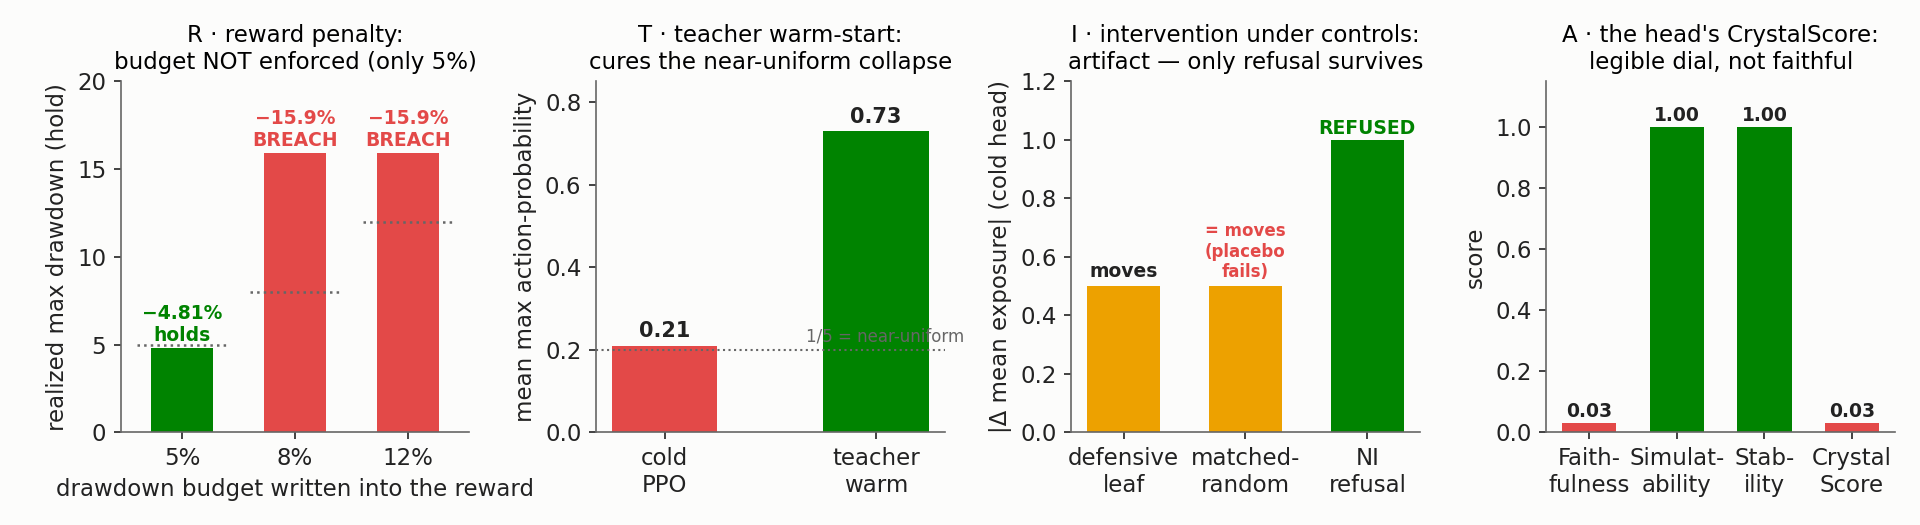
\includegraphics[width=\linewidth]{figures/fig_levers.png}
  \caption{The four levers on the real daily panel, under controls. R (Eq.~\ref{eq:reward}): the
  reward penalty holds only the $5\%$ budget ($-4.81\%$); the $8\%/12\%$ heads breach ($-15.9\%$)
  --- the penalty does not enforce the budget (the Lagrangian does, at a goal cost). T
  (Eq.~\ref{eq:bc}): the teacher warm-start cures the cold near-uniform collapse (mean max
  action-prob $0.21\to0.73$). I (Eqs.~\ref{eq:write},~\ref{eq:ni}): the control battery shows the
  intervention is NOT a clean causal control --- a matched-random leaf moves the cold head as much
  as the defensive one (placebo fails); belief-write fidelity $3\%$; only the NI \emph{refusal}
  survives. A: the cold head scores $\textsc{CrystalScore}=0.03$ ($F\,0.03\times S\,1.0\times
  S\!t\,1.0$) --- a legible, stable dial, not a faithful command surface (boundary-aware
  re-measurement: cold $F$ confirmed ${\approx}0$; warm-started heads revised to ${\approx}0.8$,
  see the correction in \S\ref{sec:levers}).}
  \label{fig:levers}
\end{figure}

\section{Real-data results}
\label{sec:results}

\subsection{The readable champion beats the best static portfolio}
\label{sec:champion}

On the flagship goal task (double the wealth in ten years, US universe, Eq.~\ref{eq:bellman}),
the dynamic readable policy beats the \emph{best static} portfolio by $+10.5$\,pp goal
probability (CI90 $[+9.3,+11.7]$, stable across folds; Figure~\ref{fig:dplift}). An 8-leaf tree
reproduces the champion's table at $0.92$ (Eq.~\ref{eq:simul}) --- a human can simulate it. A
dedicated gate checks that the lift is not bought with deeper misses; on Chinese data it
correctly caught exactly that (the digital-option behavior of goal-reaching policies), which
moved $\lambda$ into the user contract --- the tension between goal probability and miss depth
is structural, so the \emph{user} must own it. A conditional PPO challenger (behavior-cloned
from the DP teacher, hard-shielded on capacity \citep{achiam2017,schaul2015}) currently
\emph{loses} to exact DP on the same action space (regret $6.6$\,pp); we report this because
the field's default is the opposite claim.

\begin{figure}[t]
  \centering
  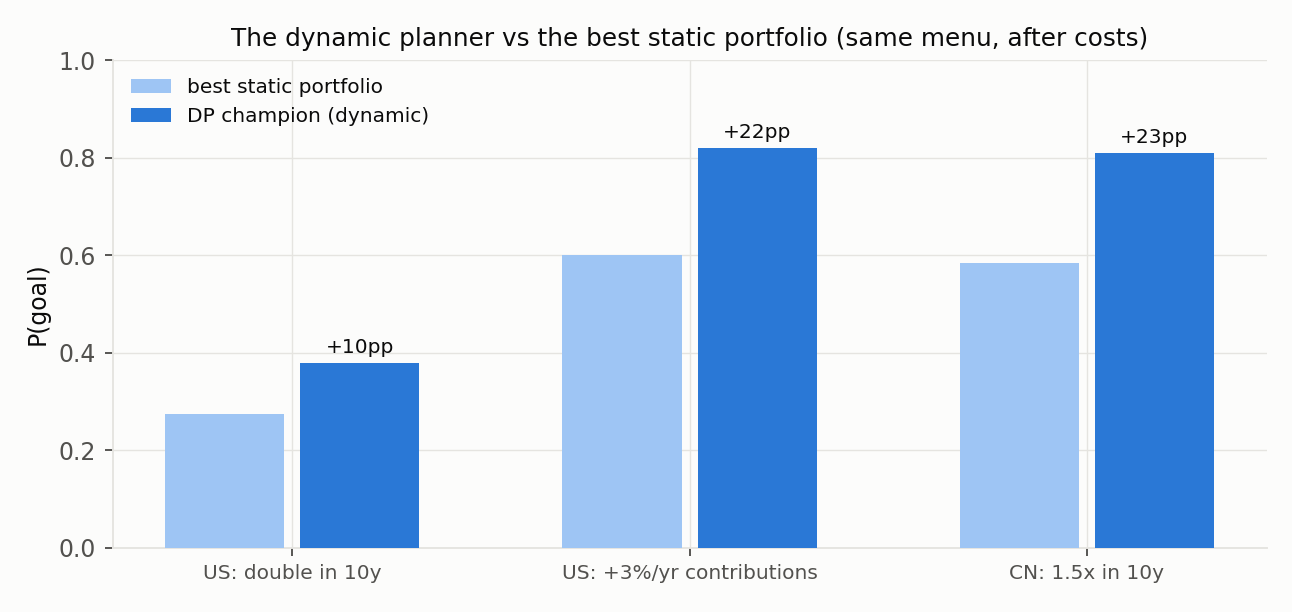
\includegraphics[width=.75\linewidth]{figures/fig_dp_lift.png}
  \caption{The readable dynamic policy vs the best static portfolio on the same menu, after
  costs (US universe; the CN panel shown for the separate-verdict discipline). The lift is
  $+10.5$\,pp goal probability on the flagship task.}
  \label{fig:dplift}
\end{figure}

\subsection{The improvement loop, profile by profile: $1\% \to 52\%$ at unchanged risk}
\label{sec:ablation}

The outer layer (the subject of the companion paper) is a loop in which an LLM coding agent
proposes typed machinery changes that must survive a control battery --- matched-random
(placebo), wrong-direction, half-dose, out-of-time --- plus a one-shot held-out read.
Here it matters as CRYSTAL-1's \emph{real-data adaptation record}: 65 iterative cycles across
five investor profiles on the US universe, acceptance on the user's declared objective $J$
(Eq.~\ref{eq:J}), every accept immediately re-read on a held-out seed.

\begin{table}[h]
\centering\small
\begin{tabular}{lcccc}
\toprule
profile & accepts/13 & $J$: cycle 0 & $J$: final (hold) & $\Prob(\text{goal})$: $0 \to$ final \\
\midrule
conservative       & 5 & $-0.007$ & $+0.497$ & $0.01 \to 0.52$ \\
mod-conservative   & 2 & $+0.114$ & $+0.398$ & $0.18 \to 0.46$ \\
moderate           & 4 & $+0.008$ & $+0.429$ & $0.06 \to 0.48$ \\
mod-aggressive     & 2 & $-0.154$ & $+0.229$ & $0.00 \to 0.35$ \\
aggressive         & 2 & $+0.079$ & $+0.252$ & $0.08 \to 0.25$ \\
\bottomrule
\end{tabular}
\caption{The per-profile improvement loop on real US data: 15 of 65 candidates accepted, all 15
confirmed on held-out data (dev $\approx$ hold; no development-seed overfitting visible). The
largest gains land exactly where the capacity filter bites hardest: the conservative profile's
goal probability rises from $1\%$ to $52\%$ at an \emph{unchanged} risk budget. All numbers are
research-tier scenario estimates under \S\ref{sec:kernels}.}
\label{tab:ablation}
\end{table}

\begin{figure}[t]
  \centering
  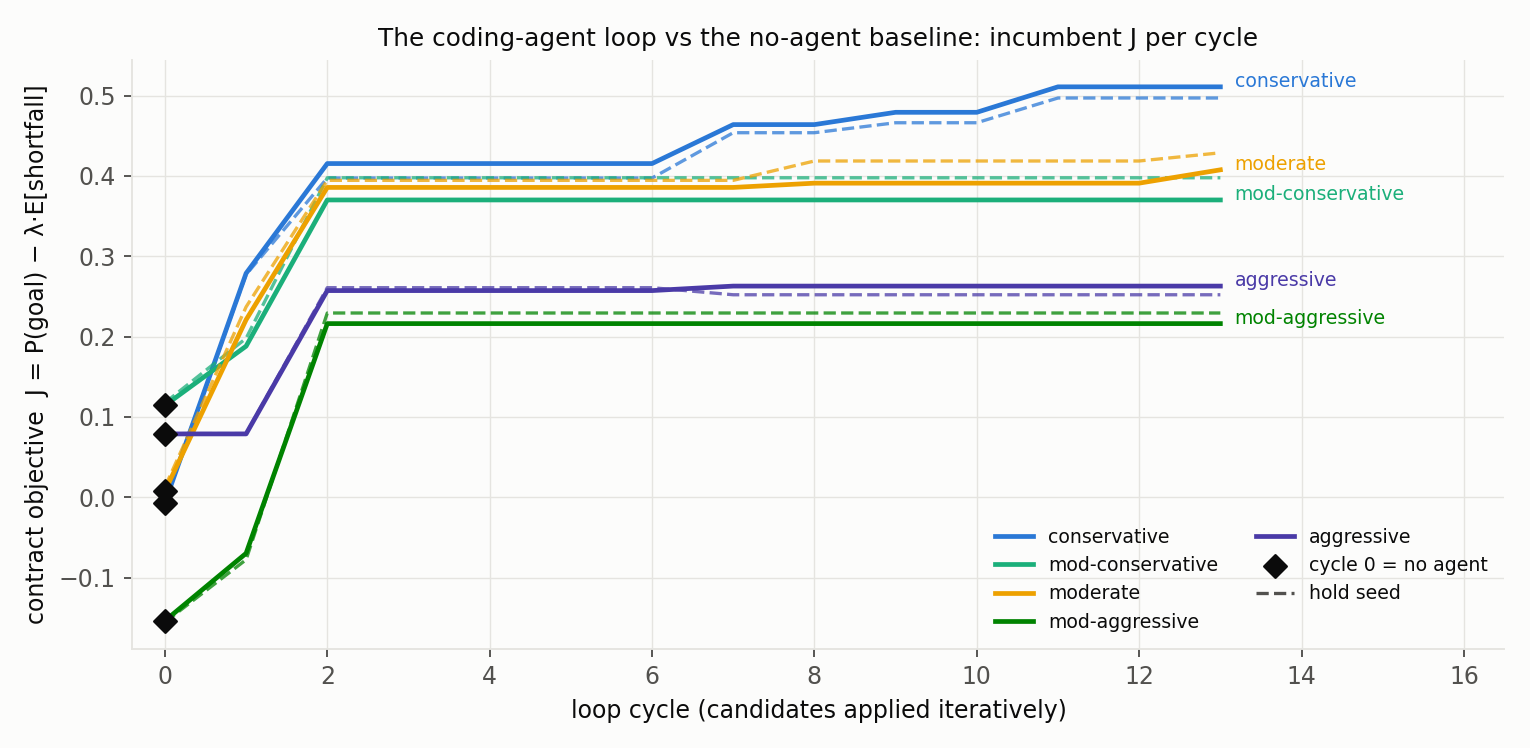
\includegraphics[width=\linewidth]{figures/fig_ablation_J.png}
  \caption{Learning curves on real US data: the contract objective $J$ (Eq.~\ref{eq:J}) vs loop
  cycle, per profile. The leftmost point (cycle 0) is the no-agent baseline; solid =
  development seed, dashed = held-out. Plateaus are honest rejections; steps are accepted
  candidates.}
  \label{fig:ablation}
\end{figure}

\subsection{The promise backtest: do the quoted floors come true?}
\label{sec:backtest}

For each profile we sweep the capacity budget across its band and, at every point-in-time
origin (semi-annual from 2010), quote the promise $F_q$ (Eq.~\ref{eq:floor}), then run the
\emph{same policy} on the realized subsequent years and score Eq.~\ref{eq:exceed}. The first
run failed the conservative profile at $48.5\%$ --- and the failure was the finding: the
promise there is cash-dominated, and level-resampled rates let pre-crisis $4$--$5\%$ yields
leak into zero-rate-era promises. The persistent-rate repair (Eq.~\ref{eq:persistentrate})
lifted exactly the diagnosed cells: conservative exceedance $48.5\% \to 84.2\%$, and \textbf{all
five US profiles now clear the $80\%$ bar} across 576 PIT cells; the risk (drawdown) promises
held in $100\%$ of all 936 cells on both markets (Figure~\ref{fig:exceedance}). China ---
evaluated separately, never averaged --- passes $1/5$ with three diagnosed mechanisms and named
fixes queued. \emph{Evidence tier, stated plainly:} the v1.4 pass re-uses the windows whose
failures motivated the fix --- development-tier by our own taxonomy; the genuine forward test
is pre-registered (first scoring read 2027-07-12; an untouched multi-year fold matures 2029).

\begin{figure}[t]
  \centering
  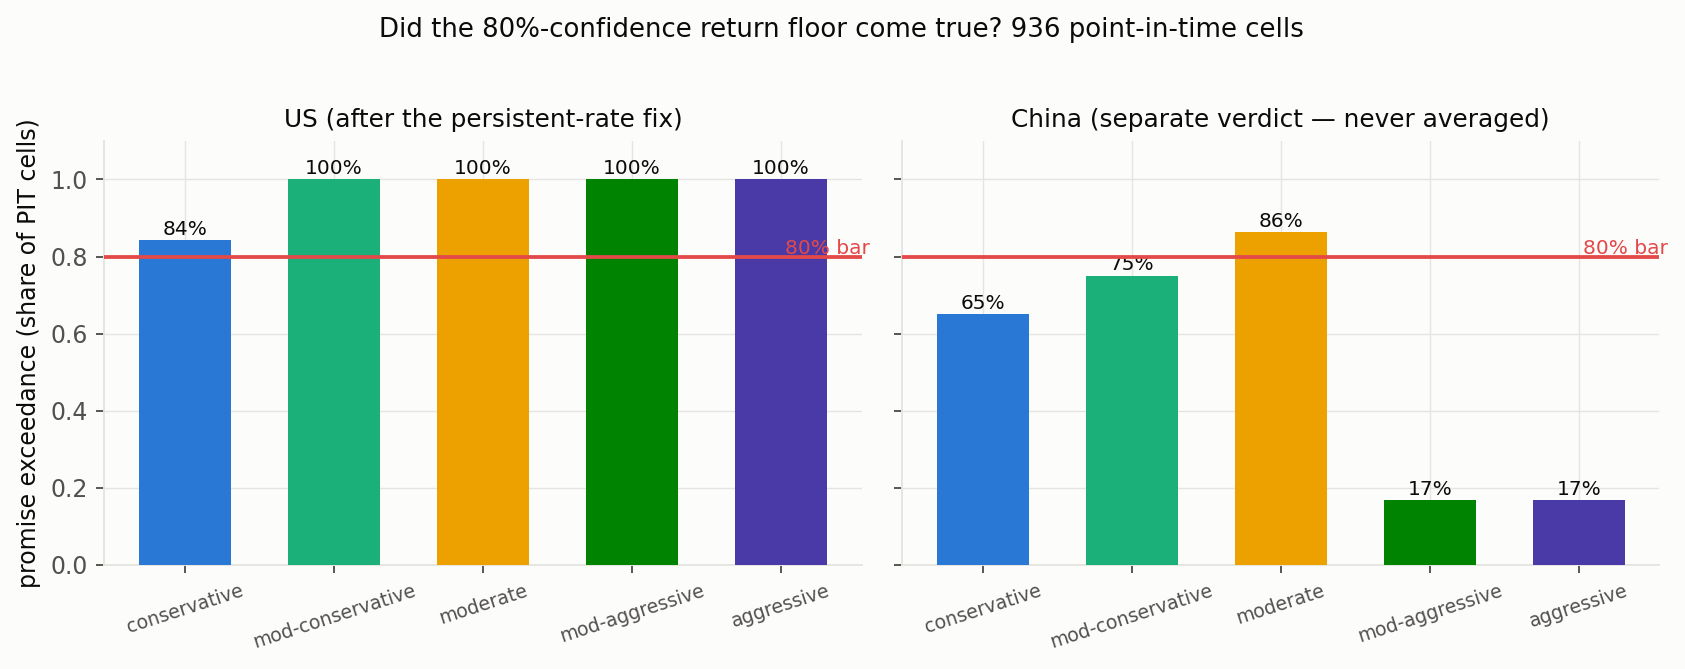
\includegraphics[width=\linewidth]{figures/fig_backtest_exceedance.png}
  \caption{Promise exceedance (Eq.~\ref{eq:exceed}) per profile against the $80\%$ bar. Left:
  US after the persistent-rate fix --- $5/5$ profiles pass. Right: China, reported separately;
  three failures with diagnosed mechanisms. Risk promises: $100\%$ of all 936 cells.}
  \label{fig:exceedance}
\end{figure}

\subsection{A certified readable rule on untouched data}
\label{sec:cert}

The loop's frozen gate has certified exactly one real-data policy to date --- and it is a
sentence (Eq.~\ref{eq:rule}). It entered with 7 accepts and \textbf{0} placebo accepts, and
held one-shot on 629 untouched trading days: Sharpe $1.46$ vs $1.39$ buy-and-hold, max drawdown
$-12.9\%$ vs $-15.5\%$, risk-adjusted improvement $z = +2.06$. The claim is a \emph{risk} claim
(same return, meaningfully less pain), certified as such; a written return-improvement rule was
separately tested and \emph{closed} ($-8.8\%$). A fully autonomous lifetime run then refined
this rule under the same gates: 40 proposals $\to$ 4 certified refinements, with the evidence
budget self-sustaining ($0.20 \to 0.40$).

\subsection{The transparency audit}
\label{sec:audit}

The certified rule's machinery was audited on the real panel: naming faithfulness $1.0$ (the
state called ``bear'' is the state in which de-risking is optimal under the world model);
10-seed behavioral stability $1.0$; rule re-discovery from scratch $3/3$; belief MDL deficit
$0.0$ (Eq.~\ref{eq:mdl}). These are the CRYSTAL-1 entries of Figure~\ref{fig:crystalscore} and
Table~\ref{tab:final}. Their honest scope: measured on one substrate and one rule family ---
hardening them across substrates, seeds and profiles is Month~1 of the research program
(\S\ref{sec:program}).
\joseph{H1 asks whether the machine-simulatability 0.92 predicts \emph{human}
simulatability --- your psychophysics.}

\begin{table}[h]
\centering\small
\begin{tabular}{p{3.4cm}p{4.6cm}p{4.9cm}}
\toprule
 & \textbf{CHRL / R6c} & \textbf{CRYSTAL-1} \\
\midrule
Memory & 64-d unnamed latent, smeared; blast radius unboundable & named posterior $b_t$
(Eq.~\ref{eq:belief}); the sole memory channel \\
Policy legibility & post-hoc codes over a continuous latent; story acc.\ $0.244$ & the policy
\emph{is} a table/rule; 8-leaf story acc.\ $0.92$ at parity \\
Steering primitive & force the latent toward a K-means centroid (correlation) & named
\emph{do}-write (Eq.~\ref{eq:write}), fidelity $1.0$ \\
Refusals & OOD gate shrinks or zeroes steps & the NI bar (Eq.~\ref{eq:ni}) refused a $+1$-nat
promotion \\
Control surface & ${\sim}214$ knobs & 5 named levers \\
Seed stability & $0.619$ & $1.00$ (10 seeds) \\
\textsc{CrystalScore} (Eq.~\ref{eq:cs}) & $\mathbf{0.151}$ & $\mathbf{0.92}$ \\
Flagship real-data result & walk-forward validation: Sharpe $1.09$, maxDD $-7.34\%$ & certified
rule, 629 untouched days: Sharpe $1.46$ vs $1.39$, maxDD $-12.9\%$ vs $-15.5\%$; DP champion
$+10.5$\,pp \\
Deployment status & deployed: live firewall, operating history & the goal machinery live on the
US universe (paper track); client certification still \emph{refused}, with dated unlocks \\
\bottomrule
\end{tabular}
\caption{The final comparison, real data only. The honest split survives in refined form: R6c
remains the longer-operating deployed system; CRYSTAL-1 wins every legibility and control axis
\emph{and} now carries its own real-data results, while its client-facing certification
correctly refuses until the pre-registered reads mature.}
\label{tab:final}
\end{table}

\section{The designed-market experiment: can a market reward only a clean mind?}
\label{sec:polygon}

Real markets have very noisy logic: the regime is largely priced, so the honest value of even a
perfect regime belief can be zero --- and a null result on real data cannot distinguish ``the
instrument is broken'' from ``there was nothing to detect.'' This motivates one deliberately
synthetic experiment, asked as a question: \emph{can one build a market that rewards only a
``clean'' mind --- an environment where the belief information carries value by construction,
so that command-surface machinery can be calibrated at all?}

We built such an environment (a regime market whose returns are generated from latent states
the belief can, in principle, track) and used it strictly as \textbf{instrument calibration} ---
none of the following is market-performance evidence. On it: belief writes were \emph{proved}
causal against an exogenous belief-MDP optimum (agreement $0.80$ corner head / $0.835$
tree head); a likelihood-based \emph{lie detector} separates sharp-but-wrong commands from
uncertain-but-right ones (excess predictive NLL $0.43$ vs ${\approx}0$; detection $0.71$ at
$5\%$ false alarms), while the na\"ive entropy gate points \emph{backwards} (it trusts the
confident lie); a 216-cell factorial showed command composition is non-additive with
\emph{sign-flipping} cross-terms (median $|\varepsilon| = 2.66$, both signs observed, surviving
raw logits) --- which is why the write surface is governed by a calibrated ledger,
$D = \sum{|\alpha_i|\tau_i} + \sum{|\varepsilon_{ij}|\tau}$, a co-activation cap
$N_{\text{live}} \le K$, a kNN manifold governor ($24/24$ engineered off-manifold corners
flagged at $1.2\%$ held-out FPR) and a writ ladder whose own false-accept rate has a first
estimate ($0/48$; $\lesssim 6\%$ by the rule of three). On a \emph{hard} designed substrate the
gate also certified a genuine return$\leftrightarrow$legibility \emph{tension} --- legibility
is not free everywhere, and anyone claiming otherwise is measuring easy tasks.

The bridge back to reality is an explicit \textbf{value-of-information gate}
(Figure~\ref{fig:polygon}): the designed market shows VoI $= 5.92$ ($+282\%$ of a belief-blind
baseline) and the gate \emph{opens}; on a real book the measured VoI is $0$ and the gate
\emph{closes} --- so nothing calibrated on the designed market is allowed to generate a
real-market claim. The one real-panel port of this command surface (a belief-driven exposure
mode) exists behind that gate and an enable table, and is deliberately \emph{not} cited as
evidence anywhere in \S\ref{sec:results}.

\begin{figure}[t]
  \centering
  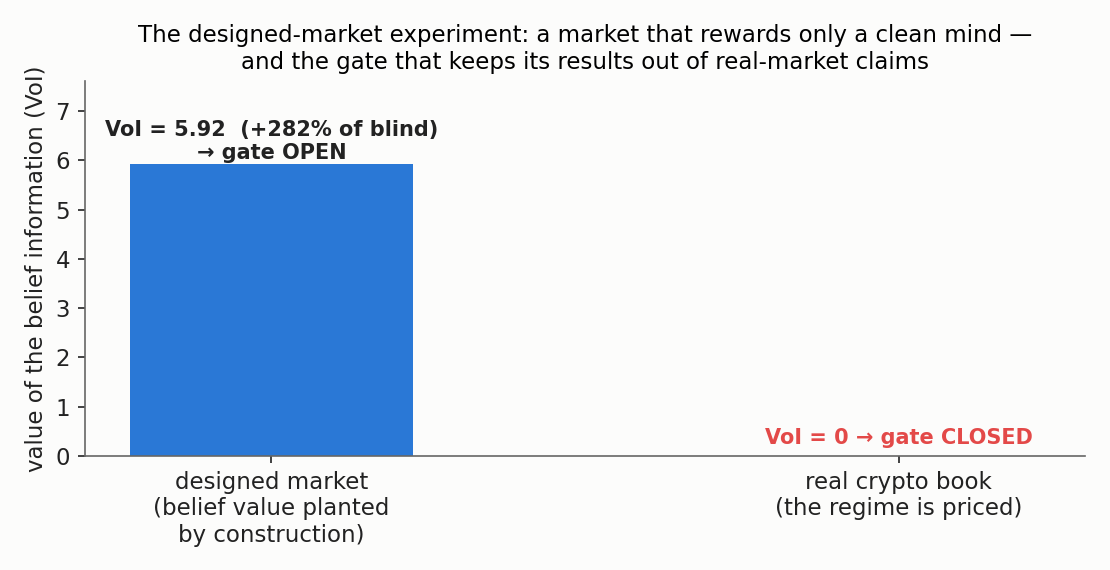
\includegraphics[width=.72\linewidth]{figures/fig_polygon.png}
  \caption{The designed-market experiment and its fence. Left: the environment built to reward
  a clean mind --- the belief information is worth $+282\%$ of blind by construction, so
  command machinery (causal writes, the lie detector, composition governance) can be
  calibrated. Right: the same measurement on a real book returns zero, and the gate closes ---
  designed-market results are instrument calibration, never market evidence.}
  \label{fig:polygon}
\end{figure}

\section{What did not work, and what bounds the claims}
\label{sec:nulls}

A paper about honest machinery should list its own falsifications; each cost us a believed
hypothesis, and the machinery that killed them is the contribution. (i) A famous valuation
indicator (\textbf{CAPE}): made real-data forecasts worse $\to$ falsified, reverted. (ii) The
\textbf{PPO challenger} loses to the readable table on real data (regret $6.6$\,pp) $\to$
reported, not hidden. (iii) A \textbf{Nasdaq-tracking sleeve} dominated every Chinese profile
$\to$ red-flagged \emph{by the agent itself}: its edge is one untestable sample era. (iv) The
\textbf{conservative promise failed its first backtest} ($48.5\%$ vs $80\%$) $\to$ the
diagnosis became Eq.~\ref{eq:persistentrate} and repaired exactly the diagnosed cells
($\to 84.2\%$). (v) A \textbf{written return-improvement rule} was tested and closed
($-8.8\%$) --- the certified claim is risk-shaped, not alpha-shaped. (vi) On a hard
\emph{designed} substrate, \textbf{legibility is provably not free} (the certified tension of
\S\ref{sec:polygon}) --- the open frontier of the interpretability track. (vii) Post-hoc
interpretability on CHRL \textbf{was not worthless}: it found the load-bearing concepts
(motifs, codes, counterfactual replay) that CRYSTAL-1 promoted from probes into architecture
--- the right summary is that building them in made the story $\sim\!4\times$ more compressible
($0.244 \to 0.92$ at the same budget).

\section{Related work}
\label{sec:related}
Interpretability-by-construction vs post-hoc explanation \citep{rudin2019,lipton2018}; rigor
and evaluation of interpretability \citep{doshivelez2017,hoffman2018}; faithfulness as a
criterion \citep{jacovi2020}. Belief-state control \citep{kaelbling1998} and regime models
\citep{hamilton1989} supply the named memory; soft trees \citep{frosst2017} the legible head;
MDL \citep{rissanen1978} the non-saturating ruler; interventional causality \citep{pearl2009}
the faithfulness protocol. Discretized latent-action behavior generation \citep{lee2024vqbet}
pursues the complementary direction --- learned discrete codes for \emph{expressiveness} ---
where CrystalRL fixes the codes to \emph{named} coordinates for legibility; goal-based
planning \citep{das2020goals,browne1999}; hierarchical RL as partial legibility
\citep{sutton1999options,bacon2017option}; PPO and constrained variants
\citep{schulman2017ppo,achiam2017}; goal-conditioned value functions \citep{schaul2015};
imitation-then-optimize \citep{ross2011dagger,rusu2016distillation}; reward shaping
\citep{ng1999shaping}; the stationary bootstrap \citep{politis1994}. The self-improvement layer
--- LLM proposers over verified evaluators \citep{romera2024funsearch,novikov2025alphaevolve,%
ma2023eureka,wang2023voyager} and the statistics of adaptive search over noisy financial
evaluators \citep{baileylopez2014dsr} --- is treated in the companion paper (\emph{Hello
Crystal}); this paper builds the object those loops are allowed to modify.
\gap{position vs concept-bottleneck models (Koh et al.\ 2020) and vs circuit-style transformer
interpretability --- one paragraph each, Joseph's lit pass.}

\section{The research program: twelve hypotheses, each with a kill test}
\label{sec:program}

This section is deliberately ambitious --- the point of a legible, steerable, self-modifying
agent is not one trading policy but a \emph{general method for keeping evolving systems
readable}. Each hypothesis is falsifiable; each names the observation that kills it.
\joseph{this program is yours to reshape: pick one hypothesis per month, or replace them with
better ones --- the kill-test discipline is the only non-negotiable.}

\begin{enumerate}
  \item \textbf{H1 --- Machine simulatability predicts human simulatability.} The $0.92$ story
        accuracy is machine-measured. \emph{Test:} psychophysics --- humans predict the
        policy's action in unseen cells of the real DP tables. \emph{Kill:} human accuracy at
        chance while machine simulatability stays at ceiling.
  \item \textbf{H2 --- A legibility scaling law.} Optimal vocabulary size $K$ tracks substrate
        behavioral complexity across real universes --- a ``Kolmogorov frontier'' for policies.
        \emph{Kill:} substrates where optimal $K$ is unrelated to measured complexity.
  \item \textbf{H3 --- The return${\leftrightarrow}$legibility tension is a substrate property,
        not an architecture property.} Prediction: the tension is maximal where the regime is
        fully priced and vanishes where belief information carries value. \emph{Kill:} tension
        persists on a designed VoI${>}0$ environment.
  \item \textbf{H4 --- Interpretability drift.} Under the self-improvement loop, naming
        faithfulness decays unless actively re-certified (semantic drift of the belief
        coordinates). \emph{Test:} track Eq.~\ref{eq:faith} across accepted loop generations on
        the real machinery. \emph{Kill:} faithfulness stays at $1.0$ over $\ge$20 accepted
        changes with no re-certification.
  \item \textbf{H5 --- Motif conservation across architectures.} CHRL's discovered primitives
        re-emerge as CRYSTAL-1 rule clauses (homologous behaviors across ``species'').
        \emph{Test:} match the frozen-test primitives to leaf semantics on the same real
        windows. \emph{Kill:} no better-than-chance correspondence.
  \item \textbf{H6 --- The write protocol is pharmacological.} \texttt{SET\_BELIEF}
        dose-response on the real panel is monotone and saturating. \emph{Kill:} non-monotone
        dose regions on any certified substrate.
  \item \textbf{H7 --- Composition governance is necessary on real data.} Sign-flipping command
        interactions (so far shown only on the designed market, off-manifold) appear on the
        real panel's visited manifold. \emph{Kill (of the premise):} on-manifold real-data
        interactions are additive --- then the ledger's $\varepsilon$ term is precautionary
        overhead.
  \item \textbf{H8 --- The lie detector generalizes.} Authority-tracks-NLL discriminates
        wrong-but-sharp commands on real panels at operationally useful rates. \emph{Kill:}
        detection at chance outside the designed market.
  \item \textbf{H9 --- $\alpha_{\text{machine}}$, full-firewall.} The $0/48$ core proxy holds
        ($\le 5\%$) when estimated through the complete real-data gate stack. \emph{Kill:}
        full-stack estimate an order worse.
  \item \textbf{H10 --- Faithful client-facing explanations.} Every ``why'' sentence shown to
        a user can be made \emph{measurably} faithful: perturb the stated reason, behavior must
        move accordingly. \emph{Kill:} explanations that pass fluency review but fail
        perturbation faithfulness at scale.
  \item \textbf{H11 --- Certified vocabulary growth.} \texttt{GROW\_K} can be run as a
        certified architectural operation: the agent learns a new regime word without semantic
        drift of the old ones. \emph{Kill:} any old-coordinate faithfulness drop after growth.
  \item \textbf{H12 --- The score applies to the improver.} CrystalScore's axes transfer to the
        \emph{coding agent's} own proposals --- interpretability of the improver, not just the
        improved. \emph{Test:} score proposal rationales against their measured effects.
        \emph{Kill:} rationale--effect agreement at chance (the LLM's stated reasons are
        confabulation --- itself a publishable result).
\end{enumerate}

\section{Limitations}
\label{sec:limits}
(i) The scenario-based probabilities of \S\ref{sec:results} remain \textsc{uncalibrated
research estimates}; the calibration gates (7/10 green) and their dated forward reads
(2027-07-12; 2029) live in the companion paper. (ii) The v1.4 promise-backtest pass re-uses the
windows whose failures motivated the fix --- development-tier evidence. (iii) The real-data
CrystalScore's simulatability axis is measured on the DP champion and the certified rule family
--- not yet on every head (Month~1 of the program). (iv) The command-surface \emph{proofs}
(causal writes vs an exogenous optimum, the lie detector, composition governance) are
designed-market calibrations (\S\ref{sec:polygon}); their real-data analogues are H6--H9.
(v) China passes $1/5$ profiles; its named fixes are queued, and no CN number is averaged into
any US claim. (vi) Execution economics beyond $10$\,bp switching costs (taxes, spreads, gaps)
are only partially bounded.

\section*{Acknowledgments and drafting discipline}
Prepared \emph{write-paper-first} \citep{eisner-paper-first}: every margin \texttt{todo} marks
a real gap. Experiments were run and logged under the repository's honesty contract --- every
entry names its null, its seed, and its worst caveat --- in the spirit of \citet{feynman1974}:
\emph{``The first principle is that you must not fool yourself --- and you are the easiest
person to fool.''} LLM coding agents (Claude, Codex) operated the loops under the stated
controls; the agents propose, the gates dispose.

\bibliographystyle{plainnat}
\bibliography{refs}

\end{document}
